\documentclass[11pt]{article}
\usepackage[utf8]{inputenc}
\usepackage[russian]{babel}
\usepackage[T1]{fontenc}
\usepackage{amssymb,amsmath,clrscode,graphicx,indentfirst}

\author{Олег Смирнов}
\title{Курс kiev-clrs -- Лекция 19. Кратчайшие пути: все пары вершин, умножение матриц, алгоритм Флойда-Маршала}
\date{25 июля 2009 г.}

\begin{document}
\maketitle
\tableofcontents
\newpage
\setlength{\parskip}{1ex plus 0.5ex minus 0.2ex}
\section{Цель лекции}
\begin{itemize}
\item Поиск кратчайших путей между всеми вершинами графа
\item Смежные задачи (транзитивное замыкание и др.)
\end{itemize}

Для поиска всех кратчайших путей в графе из одной вершины используются такие алгоритмы:
\begin{itemize}
\item ненагруженный граф
  \begin{itemize}
  \item поиск в ширину (BFS): $O(E + V)$
  \end{itemize}
\item граф с неотрицательными дугами
  \begin{itemize}
  \item алгоритм Дейкстры: $O(E + V \lg V)$
  \end{itemize}
\item общий случай
  \begin{itemize}
  \item алгоритм Беллмана-Форда $O(VE)$
  \end{itemize}
\item направленный ациклический граф
  \begin{itemize}
  \item топологическая сортировка и один проход алгоритма Беллмана-Форда: $O(V+E)$
  \end{itemize}
\end{itemize}
Алгоритм Дейкстры работает за почти линейное время, а алгоритм Беллмана-Форда -- как минимум за квадратичное.

Для того, чтоб найти кратчайшие пути из каждой вершины в кажду, нужно выполнить соответствующий алгоритм для каждой вершины, т.е. $|V|$ раз:
\begin{itemize}
\item ненагруженный граф
  \begin{itemize}
  \item поиск в ширину $|V|$ раз: $O(VE + V^2)$
  \end{itemize}
\item граф с неотрицательными дугами
  \begin{itemize}
  \item алгоритм Дейкстры $|V|$ раз: $O(VE + V^2 \lg V)$
  \end{itemize}
\item общий случай
  \begin{itemize}
  \item алгоритм Беллмана-Форда $|V|$ раз: $O(V^2 E)$
  \item известно три алгоритма, которые будут рассмотрены ниже
  \end{itemize}
\end{itemize}

\section{Кратчайшие пути между всеми парами вершин}
Для ориентированного нагруженного графа $G=(V, E)$, где $V = {1, 2, \ldots, n}$ с заданной функцией весов $w~:~E~\to~\mathbb{R}$, найти матрицу $n \times n$ кратчайших путей $\delta(i, j)$ для всех $i, j \in V$.

Идея: выполнить алгоритм Беллмана-Форда для каждой вершины. Время работы: $O(V^2 E)$. Тогда для плотного графа (в котором $n^2$ дуг), время выполнения будет $\Theta(n^4)$.

\section{Динамическое программирование}
Рассмотрим матрицу смежности $A = (a_{i j})$ размерности $n \times n$ для ориентированного графа, где
\begin{equation*}
  a_{i j} = \begin{cases}
    w(i, j), \text{ если дуга } (i, j) \in E \\
    \infty, \text{ иначе }
  \end{cases}
\end{equation*}
Для использования динамического программирования, нужно определить оптимальную подструктуру (задачи меньшего размера). Алгоритм Беллмана-Форда на каждом $i$-м шаге строит кратчайшие пути длины $i$. Это было доказано в виде леммы на предыдущей лекции.

Можно определить:
\begin{equation*}
  d_{i j}^{(m)} = \text{вес кратчайшего пути из } i \text{ в } j \text{, используя } \leqslant m \text{ дуг}
\end{equation*}
Например, при $m = 0$:
\begin{equation*}
  d_{i j}^{(0)} = \begin{cases}
    0, \text{ если } i = j \\
    \infty, \text{ если } i \neq j
  \end{cases}
\end{equation*}

Из алгоритма Беллмана-Форда известно, что начиная с $n-1$:
\begin{equation*}
  d_{i j}^{(n-1)} = d_{i j}^{(n)} = d_{i j}^{(n+1)} = \ldots = \delta(i, j)
\end{equation*}
если в графе нет циклов отрицательного веса. Т.е. ответ будет получен не более чем за $n$ итераций.

Формула для рекурсивного вычисления $d_{i j}^{(m)}$:
\begin{equation*}
  d_{i j}^{(m)} = \min_k\{d_{i k}^{(m-1)} + a_{k j}\}
\end{equation*}
\begin{figure}[ht!]
  \centering
  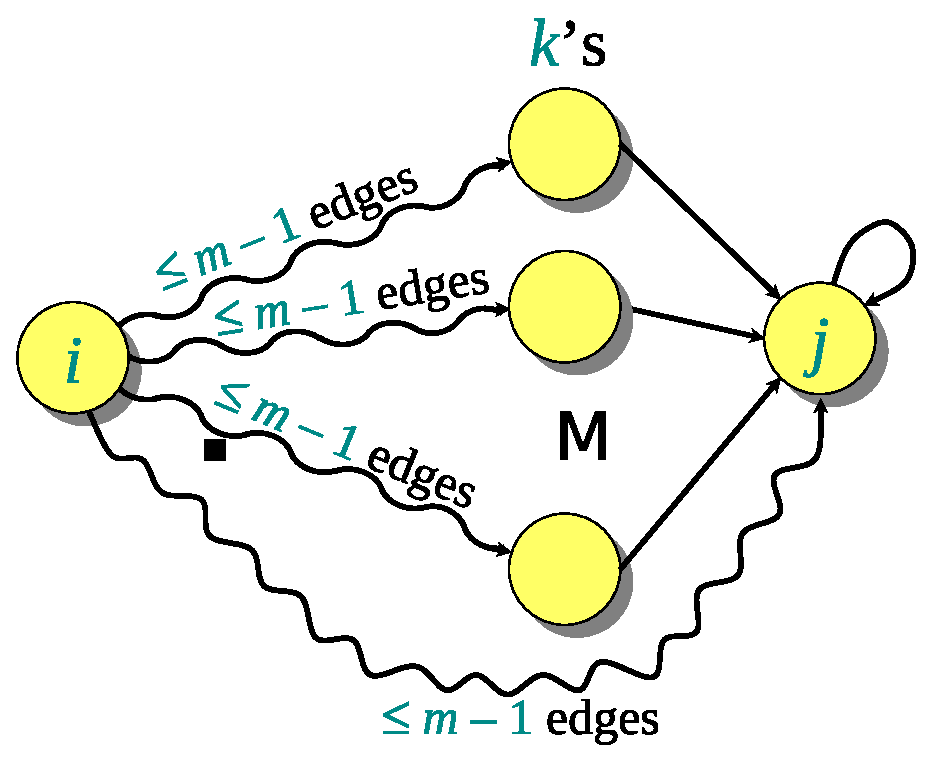
\includegraphics[width=2.5in]{lecture19/bford.eps}
  \caption{Алгоритм Беллмана-Форда}
\end{figure}
Очевидно, что формула перебирает все возможные пути в $j$, рассматривая только смежные вершины. Если существуюет путь без промежуточной смежной вершины (длиной $m-1$), то он тоже будет рассмотрен, т.к. вес дуги из $j$ в $j$ считается равным $0$.

Алгоритм является очередным примером использования релаксации:
\begin{codebox}
\Procname{$\proc{N\_Bellman\_Ford}(G, w)$}
\li \For $m \gets 1$ \To $n-1$
\li \Do \For $i \gets 1$ \To $n$
\li        \Do \For $j \gets 1$ \To $n$
\li            \Do \For $k \gets 1$ \To $n$
\li                \Do \If $d_{i j} > d_{i k} + a_{k j}$ \Comment шаг релаксации
\li                    \Then $d_{i j} \gets d_{i k} + a_{k j}$
                   \End
               \End
            \End
        \End
    \End
\li \Return $d$
\end{codebox}
Время работы: $O(n^4)$, т.е. такое же, как и у алгоритма Беллмана-Форда в худшем случае.

\section{Умножение матриц}
Алгоритм поиска кратчайших путей можно улучшить с помощью умножения матриц.

Для матриц $C$, $A$ и $B$ размера $n \times n$, произведение $C = A \cdot B$:
\begin{equation*}
  c_{i j} = \sum^n_{k=1}a_{i k}b_{k j}
\end{equation*}
выполняется за время $\Theta(n^3)$ стандартным алгоритмом.

Если заменить операцию сложения ``$+$'' на взятие минимума ``$\min$'', а умножение ``$\cdot$'' на ``$+$'', то можно формула умножения
\begin{equation*}
  c_{i j} = \min_k\{a_{i k} + b_{k j}\}
\end{equation*}
будет иметь такую же форму, как
\begin{equation*}
  d_{i j}^{(m)} = \min_k\{d_{i k}^{(m-1)} + a_{k j}\}
\end{equation*}

Таким образом, вычисление матрицы путей можно представить в виде:
\begin{equation*}
  D^{(m)} = D^{(m-1)} \otimes A
\end{equation*}

Единичная матрица:
\begin{equation*}
  A^0 = I = \left( \begin{smallmatrix} 
    0 & \infty & \infty & \infty \\
    \infty & 0 & \infty & \infty \\
    \infty & \infty & 0 & \infty \\
    \infty & \infty & \infty & 0 \\
  \end{smallmatrix} \right) = D^0 = (d_{i j}^{(0)})
\end{equation*}

Операция $\otimes$ обладает свойством \textbf{ассоциативности}, т.к. $(\mathbb{R}, \min, +)$ -- \textbf{замкнутое полукольцо}, $(\mathbb{R}, \min)$ -- коммутативный моноид, $(\mathbb{R}, +)$ -- моноид.

Вычисление матрицы путей $D$ является возведением в степень матрицы $A$:
\begin{align}
  D^{(1)} = D^{(0)} \otimes A = A^1 \\
  D^{(2)} = D^{(1)} \otimes A = A^2 \\
  \ldots \\
  D^{(n-1)} = D^{(n-2)} \otimes A = A^{n-1} \\
  D^{(n-1)} = (\delta(i, j)) 
\end{align}

Время работы: $\Theta(n\cdot n^3) = \Theta(n^4)$ -- такое же как и для $n$ вызовов Беллмана-Форда.
\section{Улучшенный алгоритм умножения матриц}
Использовать алгоритм Страссена в этом случае нельзя, т.к. этот алгоритм использует вычитание -- обратную операцию к сложению. В полукольце $(\mathbb{R}, \min, +)$ обратной операции для $\min$ не существует (иначе это было бы кольцо).

Однако можно использовать возведение в степень методом ``разделяй-и-властвуй'' -- последовательное возведение в квадрат.

Необходимо вычислить
\begin{equation*}
  A^{2^{\lceil \lg(n-1) \rceil}}
\end{equation*}
так как $A^{n-1} = A^n = A^{n+1} = \ldots$.

Это можно сделать за $\Theta(n^3 \lg n)$ итераций. Чтоб обнаружить циклы отрицательного веса, после выполнения алгоритма нужно проверить диагональ на наличие отрицательных чисел. Это можно сделать за время $O(n)$. 
\section{Алгоритм Флойда-Уоршелла}
Решение динамическим программированием можно сделать еще лучше. Идея в том, чтоб определить подзадачи более эффективным способом. Вместо вычисления минимума из $k$ значений, можно вычислять минимум из двух. Тогда время работы алгоритма станет кубическим.

Пусть $c_{i j}^k$ -- вес кратчайшего пути из $i$ в $j$, используя только вершины из множества $\{1, 2, \ldots, k\}$.

Тогда $\delta(i, j) = c_{i j}^{(n)}$ и $c_{i j}^{(0)} = a_{i j}$.

На шаге релаксации проверяется условие: станет ли путь из $i$ в $j$ короче, если в него добавить промежуточную вершину с номером $k$?
\begin{equation*}
  c_{i j}^{(k)} = min_k \{c_{i j}^{(k-1)}, c_{i k}^{(k-1)} + c_{k j}^{(k-1)}\}
\end{equation*}
\begin{figure}[ht!]
  \centering
  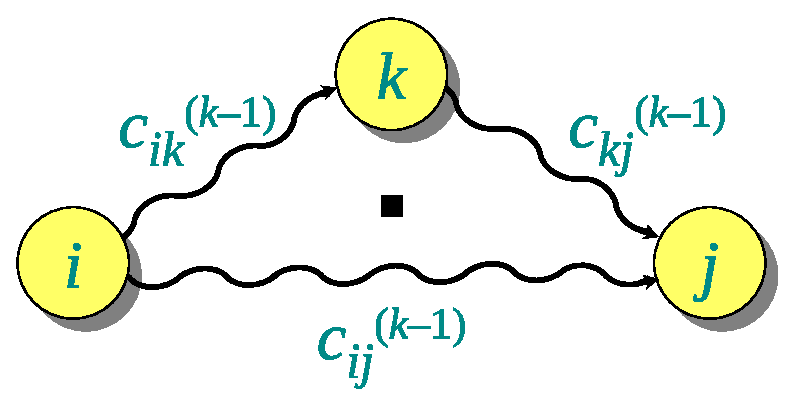
\includegraphics[width=2.5in]{lecture19/fwarshall.eps}
  \caption{Алгоритм Флойда-Уоршелла}
\end{figure}
Все промежуточные вершины на рисунке -- из множества $\{1, 2, \ldots, k\}$.

\begin{codebox}
\Procname{$\proc{Floyd\_Warshall}(G, w)$}
\li $C \gets A$
\li \For $k \gets 1$ \To $n$
\li \Do \For $i \gets 1$ \To $n$
\li        \Do \For $j \gets 1$ \To $n$
\li            \Do \If $c_{i j} > c_{i k} + c_{k j}$ \Comment шаг релаксации
\li                \Then $c_{i j} \gets c_{i k} + c_{k j}$
               \End
            \End
        \End
    \End
\li \Return $d$
\end{codebox}

Алгоритм выполняется за $\Theta(n^3)$ итераций и весьма эффективен на практике. В случае, если граф не плотный, алгоритм намного лучше Беллмана-Форда. Отрицательный циклы графа можно обнаружить2, например, выполнив еще один раунд алгоритма.
\section{Транзитивное замыкание графа}
Необходимо найти транзитивное замыкание графа, т.е. вычислить матрицу $T$, где
\begin{equation*}
  t_{i j} = \begin{cases}
    1, \text{ если есть путь из } i \text{ в } j \\
    0, \text{ иначе}
  \end{cases}
\end{equation*}

Можно выполнить алгоритм Флойда-Уоршелла, используя операции $(\vee, \wedge)$ вместо $(\min, +)$:
\begin{equation*}
  t_{i j}^{(k)} = t_{i j}^{(k-1)} \vee (t_{i k}^{(k-1)} \wedge t_{k j}^{(k-1)})
\end{equation*}

Время выполнения: $\Theta(n^3)$. Т.к. операции образуют кольцо на множестве элементов $\{0, 1\}$, можно использовать алгоритм Страссена, который выполняется за субкубическое время.
\section{Алгоритм Джонсона}
Алгоритм Дейкстры очень удобен для получения всех кратчайших путей в графе, т.к. для $n$ вершин он выполняется за: $O(VE + V^2 \lg V)$ -- почти квадратичное время. Для его использования нужно предварительно избавиться от дуг отрицательного веса.

Просто добавить к весу каждой дуги некоторую константу не получится, т.к. разные пути содержат разное количество дуг. Вместо этого можно назначить ``вес'' каждой вершине.

Теорема: используя функцию $h: V \rightarrow \mathbb{R}$, можно ``перевзвесить'' каждую дугу $(u, v) \in E$ задав $w_h(u, v) = w(u, v) + h(u) - h(v)$. Тогда для любых двух вершин все пути между ними будут ``перевзвешены'' на одинаковое значение.

Пусть $p = v_1 \rightarrow v_2 \rightarrow \ldots \rightarrow v_k$ -- путь в графе $G$. Тогда:
\begin{align*}
  w_h(p) = \sum_{i=1}^{k-1} w_h(v_i, v_{i+1}) = \\
  = \sum_{i=1}^{k-1} (w(v_i, v_{i+1}) + h(v_i) - h(v_{i+1})) = \\
  = \sum_{i=1}^{k-1} w(v_i, v_{i+1}) + h(v_1) - h(v_k) = \\
  = w(p) + \underbrace{h(v_1) - (v_k)}_{\text{константа} \geqslant 0}
\end{align*}

Следствие:
\begin{equation*}
  \delta_h(u, v) = \delta(u, v) + h(u) - h(v)
\end{equation*}

Если найти функцию $h: V \rightarrow \mathbb{R}$, такую, что $w_h(u, v) \geqslant 0$ для всех $(u, v) \in E$, то можно выполнить алгоритм Дейкстры для каждой вершины графа с измененными весами. Функция должна сделать веса всех дуг неотрицательными.

Можно заметить, что:
\begin{equation*}
  w_h(u, v) \geqslant 0 \iff h(v) - h(u) \leqslant w(u, v)
\end{equation*}

Эта задача разностных ограничений (частный случай задачи линейного программирования), которую можно решить с помощью алгоритма Беллмана-Форда.

Схема алгоритма Джонсона:
\begin{enumerate}
\item Найти функцию $h: V \rightarrow \mathbb{R}$ такую, что $w_h(u, v) \geqslant 0$ для всех $(u, v) \in E$. Это можно сделать с помощью алгоритма Беллмана-Форда, решив задачую разностных ограничений $h(v) - h(u) \leqslant w(u, v)$.
  \begin{itemize}
  \item Время: $O(V E)$
  \end{itemize}
\item Выполнить алгоритм Дейкстры, используя функцию $w_h$ для каждой вершины $u \in V$, чтобы вычислить $\delta_h(u, v)$ для всех $v \in V$.
  \begin{itemize}
  \item Время: $O(V E + V^2 \lg V)$
  \end{itemize}
\item Для всех $(u, v) \in V \times V$ вычислить $\delta(u, v) = \delta_h(u, v) - h(u) + h(v)$
  \begin{itemize}
  \item Время: $O(V^2)$
  \end{itemize}
\end{enumerate}

Тогда общее время работы алгоритма Джонсона: $O(V E + V^2 \lg V)$ -- практически квадратичное.

Алгоритм работает только для графов, в которых нет циклов отрицательного веса.
\end{document}
